\section{Početni zaslon i glavna navigacija}

Nakon uspješne prijave na mobilnoj aplikaciji, korisnik pristupa početnom zaslonu koji je dizajniran kao personalizirana kontrolna ploča. 

\begin{figure}[H]
    \centering
    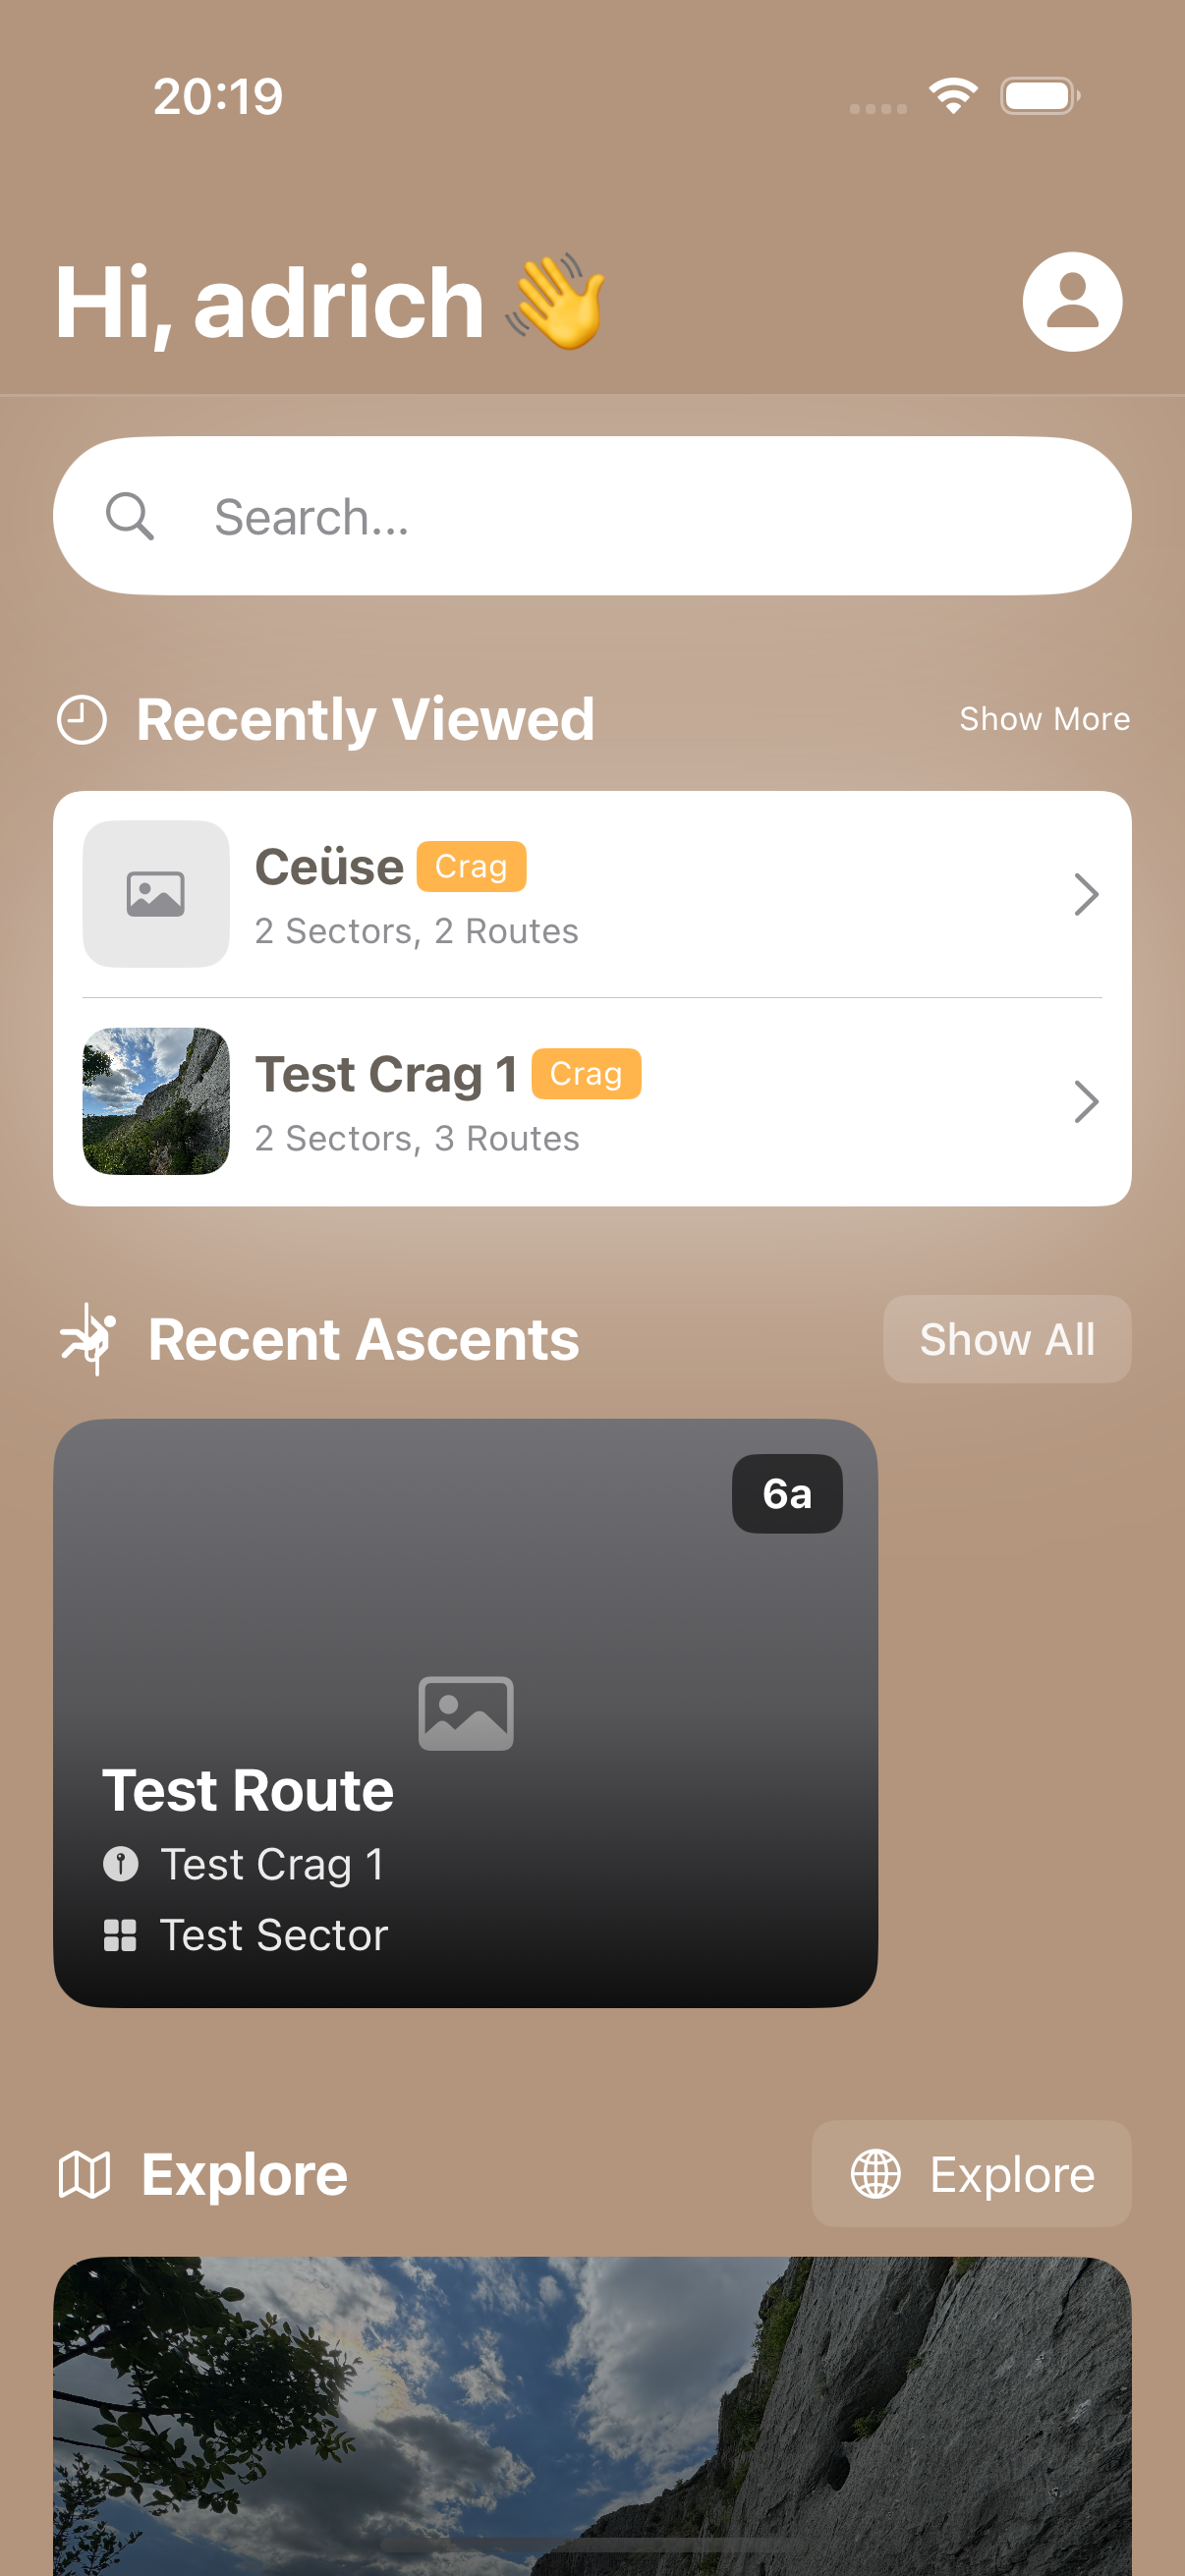
\includegraphics[width=0.35\textwidth]{images/implementacija/main_nav_1.png}
    \caption{Navigacijski zaslon aplikacije "Alpinity"}
    \label{fig:početni_zaslon}
\end{figure}

Ovaj zaslon omogućuje brzi pristup najvažnijim informacijama i funkcionalnostima. Zaslon je organiziran u nekoliko cjelina.

Na vrhu zaslona nalazi se personalizirana dobrodošlica, gumb korisničkog profila te istaknuto polje za pretraživanje koja omogućuje brzu i direktnu pretragu svih penjačkih lokacija, sektora i penjačkih smjerova. Klikom na gumb korisničkog profila korisnik odlazi na detalje svojeg profila.

Sekcija "Nedavno pregledano" (eng. \textit{Recently viewed}) nudi brze poveznice na detalje penjačke lokacije, sektore, penjačke smjerove i drugih korisnika koje je korisnik posljednje pregledavao. Korisnik ima opciju "Vidi više" (eng. \textit{View more}) koja nudi korisniku prikaz više poveznica koje je posjetio.

Odmah ispod, u sekciji "Nedavni usponi" (eng. \textit{Recent ascents}) nalazi se lista najnovijih uspona korisnika zabilježenih u dnevniku uspona. Pritiskom na određeni element liste odlazi se na detalje tog penjačkog smjera. Klikom na "Pokaži sve" (eng. \textit{Show all}) korisnik odlazi na vlastiti profil gdje su zapisani svi njegovi usponi. 

Na dnu zaslona nalazi se sekcija "Istraži" (eng. \textit{Explore}) namijenjena otkrivanju novih penjačkih destinacija kroz prijedloge popularnih lokacija. Preporuke su određene u odnosu na prijašnje korisnikove uspone, specifično preporuke su penjačke lokacije koje se nalaze u blizini lokacija koje je korisnik nekada posjetio. Klikom na određenu penjačku lokaciju u listi odlazi se na pregled detalja te lokacije. Pritiskom na gumb "Istraži" (eng. \textit{Explore}) korisnik odlazi na prikaz geografske karte sa penjačkim lokacijama.

Na web aplikaciji ne postoji ekvivalent za početni zaslon mobilne aplikacije, već poveznice na nedavno pregledane entitete nalaze se u sklopu pretraživanja. Nedavni usponi su dostupni u sklopu stranice korisničkog profila, a "Istraži" sekcija je pretvorena u zasebnu stranicu koja sadrži geografsku kartu sa penjačkim lokacijama i prijedlozima popularnih lokacija.

\begin{figure}[H]
    \centering
    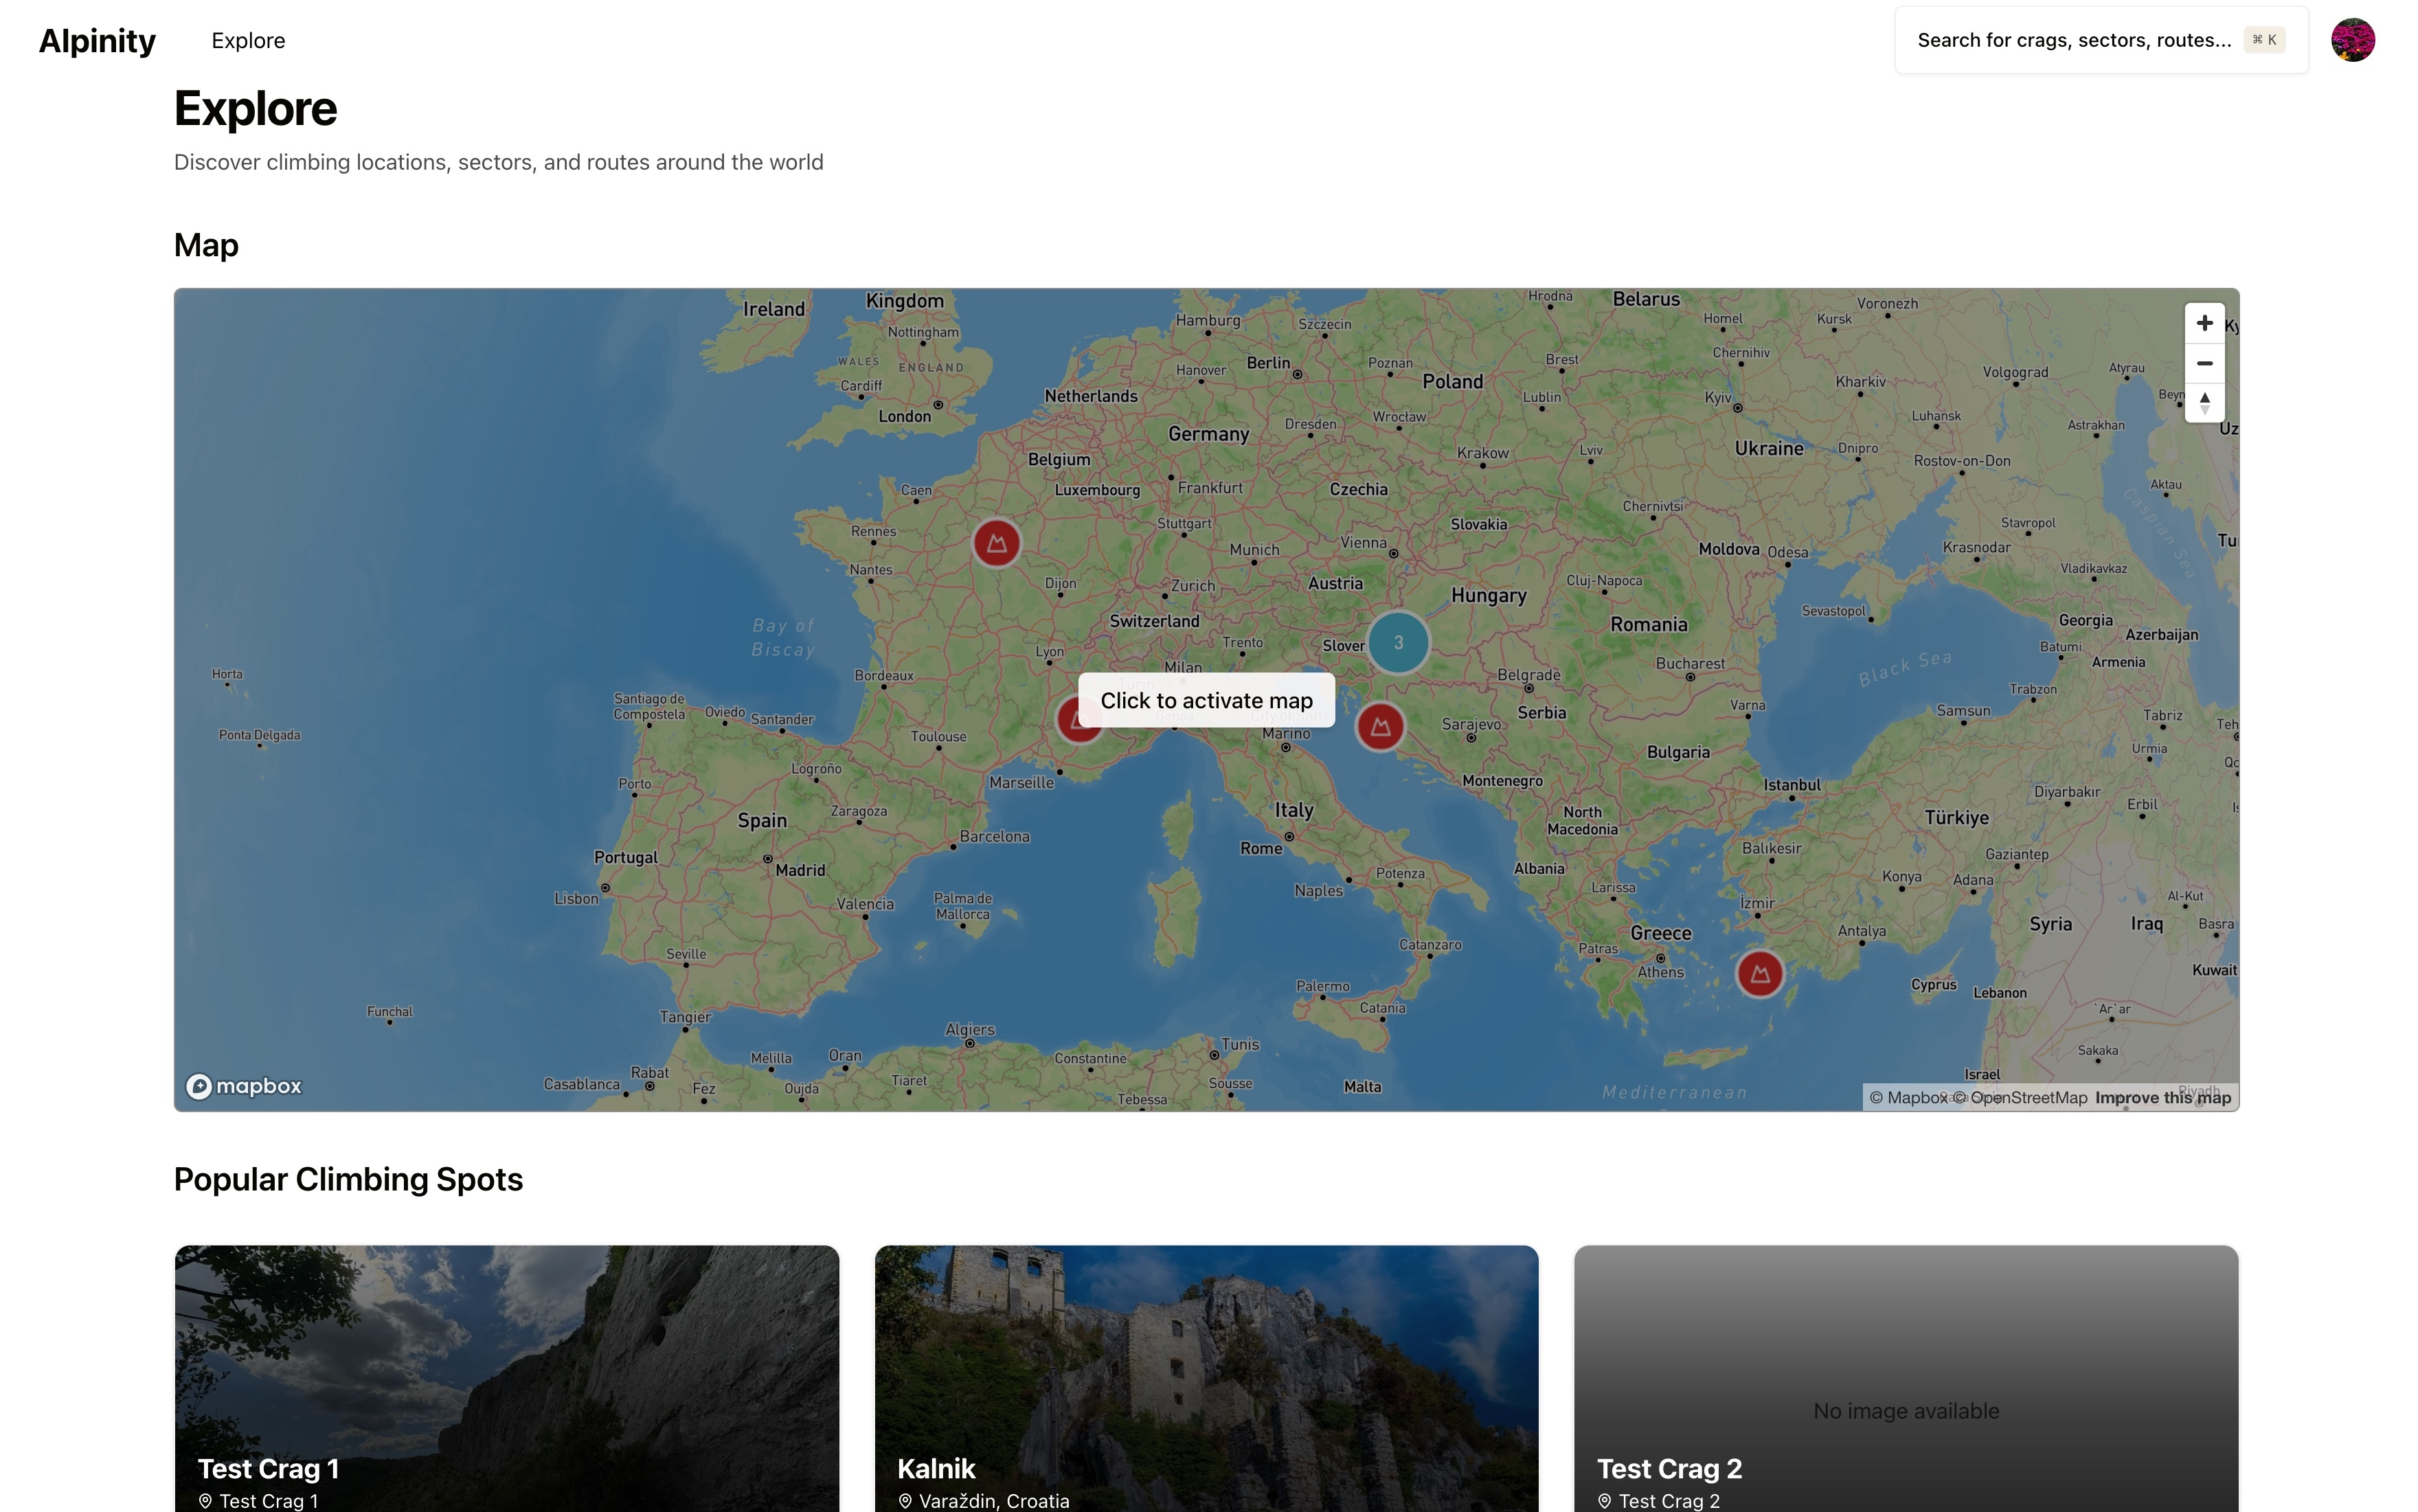
\includegraphics[width=0.9\textwidth]{images/implementacija/web/explore.jpeg}
    \caption{"Istraži" stranica web aplikacije "Alpinity"}
    \label{fig:istrazivanje_web}
\end{figure}